%%%%%%%%%%%%%%%%%%%%%%%%%%%%%%%%%%%%%%%%%
% Structured General Purpose Assignment
% LaTeX Template
%
% This template has been downloaded from:
% http://www.latextemplates.com
%
% Original author:
% Ted Pavlic (http://www.tedpavlic.com)
%
% Note:
% The \lipsum[#] commands throughout this template generate dummy text
% to fill the template out. These commands should all be removed when 
% writing assignment content.
%
%%%%%%%%%%%%%%%%%%%%%%%%%%%%%%%%%%%%%%%%%

\documentclass{article}

\usepackage{fancyhdr} % Required for custom headers
\usepackage{lastpage} % Required to determine the last page for the footer
\usepackage{extramarks} % Required for headers and footers
\usepackage{graphicx} % Required to insert images
\usepackage[utf8]{inputenc}

% Margins
\topmargin=-0.45in
\evensidemargin=0in
\oddsidemargin=0in
\textwidth=6.5in
\textheight=9.0in
\headsep=0.25in 

\linespread{1.1} % Line spacing



\setlength\parindent{0pt} % Removes all indentation from paragraphs

%----------------------------------------------------------------------------------------
%	DOCUMENT STRUCTURE COMMANDS
%	Skip this unless you know what you're doing
%----------------------------------------------------------------------------------------

% Header and footer for when a page split occurs within a problem environment
\newcommand{\enterProblemHeader}[1]{
\nobreak\extramarks{#1}{#1 continued on next page\ldots}\nobreak
\nobreak\extramarks{#1 (continued)}{#1 continued on next page\ldots}\nobreak
}

% Header and footer for when a page split occurs between problem environments
\newcommand{\exitProblemHeader}[1]{
\nobreak\extramarks{#1 (continued)}{#1 continued on next page\ldots}\nobreak
\nobreak\extramarks{#1}{}\nobreak
}

\setcounter{secnumdepth}{0} % Removes default section numbers
\newcounter{homeworkProblemCounter} % Creates a counter to keep track of the number of problems

%----------------------------------------------------------------------------------------
%	NAME AND CLASS SECTION
%----------------------------------------------------------------------------------------

\newcommand{\lessonNumber}[1]{Lezione\ \##1} % Assignment title
\newcommand{\lessonDate}[4]{#1,\ #2\ #3\ #4} % Due date
\newcommand{\lessonCourse}[1]{#1} % Course/class
\newcommand{\lessonTime}[1]{#1} % Class/lecture time
\newcommand{\lessonTeacher}[1]{#1} % Teacher/lecturer
\newcommand{\lessonAuthor}[1]{#1} % Your name


\begin{document}

\section{Premesse al Corso(1)}

Il software, se utile, ha vita lunga.
Il ruolo di un informatico è "al contorno della programmazione", in modo da non produrre codice usa e getta; deve \textbf{mantenere} il software e il codice. Tutte le attività hanno un costo e non possono essere buttate al vento.

\textbf{Engineering}, ingegnere e scienziato; l'ingegnere è colui che dai principi scientifici ne trae una finalità concreta (pratica).\textit{ La scienza deve scoprire questi principi, prepararli. L'ingegnere, sapendo che la scienza esiste, la applica. Crea qualcosa che sia manutenibile nel tempo.}

\textbf{Software}, è un terreno molto giovane, nato nella seconda guerra mondiale (40 – 45). Il \textit{SWE} molto dopo.
\textbf{SWE:} \fbox{\textbf{Def 1}l'insieme di regole e procedure di loro attuazione che vanno conosciute all'origine e applicate. }\\
\fbox{\textbf{Def 2} L'approccio \textbf{sistematico}, \textbf{disciplinato} e \textbf{quantificabile} allo sviluppo, uso, manutenzione e ritiro del software.} Non è un ramo di \textit{computer science} \textit{ramo della scienza che spiega perché i computer sono utili} ma è una disciplina ingegneristica che mette insieme elementi e conoscenze.

\begin{itemize}

	\item \textbf{Informatica},si vuole che un buon ingegnere del software conosca TUTTE le competenze informatiche;
	\item \textbf{Matematica}, scienza di base che aiuta a risolvere problemi;
	\item \textbf{Scienze gestionali ed economia}, è un attività di gruppo, correlazionale, capire come gestire risorse, tempo, denaro, cogestire;
	\item \textbf{Ingegneria}, è un pezzo di un sistema complesso che passa informazioni.
	\item \textbf{Psicologia}, il sw è rilasciato con interfacce molto orientate alle persone, bisogna intercettare le aspettative di chi usa il sw.

\end{itemize}

\textbf{Ciclo di vita di un software:} \fbox{\textbf{Def} Stati che il prodotto assume dal concepimento al ritiro}.Il sw spende la maggior parte del suo tempo nello stato di manutenzione(correttiva, adattativa, evolutiva) in cui si possono correggere degli errori e cambiare lo stato. Noi vorremmo una manutenzione che sia il meno invasiva possibile.\\

\textbf{Efficienza}\fbox{ \textbf{Def} Inversamente proporzionale alla quantità di risorse impiegate nell'esecuzione delle attività richieste.}	\\

\textbf{Efficacia}\fbox{\textbf{Def} Misura della conformità rispetto alle norme vigenti.} Si è efficaci se si raggiunge con rapidità l'obiettivo; non misura le risorse.

Il goal è massimizzare sia l'efficacia che l'efficienza, per farlo
\textbf{Best Practice }\\
\fbox{\textbf{Def} Prassi che per esperienza o per studio mostra di garantire i migliori risultati.}\\

\textbf{SWE:} L'approccio \textbf{sistematico}, \textbf{disciplinato} e \textbf{quantificabile} allo sviluppo, uso, manutenzione e ritiro del software:

\begin{itemize}
	\item \textbf{Sistematico:} agisco secondo un sistema, affronto il medesimo problema sempre nello stesso modo (best); niente improvvisazione o creatività.
	\item \textbf{Disciplinato:} la SWE è una disciplina collaborativa. Seguire in modo rigoroso la disciplina, produce affidabilità.
	\item \textbf{Quantificabile:} le azioni che compiamo seguendo i due principi precedenti devono essere quantificabili in Efficacia ed Efficienza a priori(proattivamente).
\end{itemize}


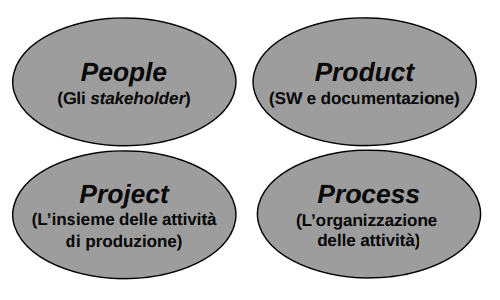
\includegraphics[width=0.75\columnwidth]{img1} % Example image 
\\

\textbf{SWE != PROGRAMMING}, la programmazione è solo un elemento, il meno importante e non può essere creativa.

\end{document}